\section{Tecnologias para Machine Learning}
\label{sec:tech-ml}

Machine Learning é uma área que vem sendo explorada e aprimorada por cientistas tanto da iniciativa privada 
como pública e acadêmica. Com a rápida evolução, onde são desenvolvidas novas tecnologias para o desenvolvimento
de métodos e algoritmos de machine learning, para ilustrar melhor é possível  dividir estas tecnologias em categorias, são elas
\textbf{linguagens de programação} e \textbf{\textit{frameworks}}, \textbf{ferramentas} e \textbf{serviços na nuvem}. 

\subsection{Principais linguagens de programação e frameworks}
\label{subsec:ling-prog}

É possível desenvolver um algoritmo utilizando qualquer linguagem de programação, mas é de grande importância que entenda as implicações
em relação á escalabilidade, performance, sintaxe e paradigmas atendidos pela linguagem escolhida. 

Muitos desenvolvedores optam por desenvolver um algoritmo com a linguagem a qual possuem mais familiaridade, 
porém dependendo da linguagem pode haver algumas caracteristicas que  oneram a performance, como por exemplo linguagens que possuem 
\textit{Garbage Collectors} \footnote{\textbf{\textit{Garbage collector}} é um mecanismo que verifica espaços alocados na memoria que não estão mais sendo utilziados e os remove.} como Java, C\#, Python entre outras. É aconselhavel que o desenvolvedor válide a 
idéia com protótipos desenvolvidos com a linguagem que possua mais familiaridade, isto torna o processo mais rápido, porém é necessário
validar se deverá refazer o código para produção em uma outra linguagem mais performática, pois em alguns casos não à necessidade
de reescrever o código em outra linguagem se o protótipo atender os critérios desejados de performance e escalabilidade. 

A linguagem de programação não influenciará no resultado final do algoritmo, porém influencia no tempo de desenvolvimento e 
velociade de processamento, alguns critérios comuns são adotados na escolha:

\begin{alineas}
    \item Sintaxe, tem influência direta na manuntenção e entendimento do código, uma boa sintaxe torna mais fácil a evolução e melhora do algoritmo;
    \item Funcionalidades dentro da linguagem, como polimorfismo, estruturas de dados como \textbf{\textit{hash tables}}, etc. 
		  Estas podem melhorar a produtividade; 
    \item Bibliotecas e frameworks disponíveis, é interessante que exista bibliotecas de estatística, de álgebra, gráficas, \textit{I/O} e grafos. Para que
          o desenvolvedor não se preocupe em fazer algo que esteja disponível, 
		  e utilizar funções de cálculos ou leituras de uma imgem prontas, e foque no algoritmo de aprendizado; e
    \item Familiaridade, não somente a do desenvolvedor mas de toda pessoa que possa ver o código.     
\end{alineas}

Foi realizada uma pesquisa em 2015 pela \textbf{KDNuggets} \footnote{\textbf{KDNuggets} é um site muito famoso nas áreas de Big Data, Data Mining e Data Science.}, para identificar qual a linguagem mais popular dentre os desenvolvedores de algortimos para 
machine learning, a ~\autoref{fig:poll-lang} mostra o resultado da pesquisa, constatou-se que a linguagem \textbf{R} é a mais utilizada seguida de 
\textbf{Python}.   


A linguagem \textbf{R} é mais utilizada para estes tipos algortimos porque foi projetada para computação estatistica, portanto 
nativamente possui muitas funções uteis para cálculos estatisticos e processamento de muitos dados, é 
altamente escalável oque é otimo para mineração de dado em uma grande massa de dados, além de possuir um grande repositório com 
bibliotecas que facilitam a aplicação da maioria dos tipos de algoritmos para machine learning e testes estatisticos o 
\textbf{CRAN}(\textit{Comprehensive R Archive Network}). 
Possui uma sintaxe elegante para transfomar dados, expressar relacionamentos e é muito fácil criar operações paralelas.
\textbf{CRAN} é um repositório de bibliotecas para a linguagem \textbf{R}, atualmente(2016) possui 9481 bibliotecas ativas, 
onde parte são focadas em machine learning.


Porém \textbf{Python} é uma linguagem mais generalista, atendendo diversos tipos de desenvolvimento como web, descktop e serviços, 
é tambem uma linguagem de script ou seja e interpredada em tempo de execução e não compilada. 
Isto fez com que ficasse muito popular entre os cientistas de dados e engenheiros de machine learning, mesmo que diferente de 
\textbf{R} não possua nativamente funções estatisticas existem bibliotecas que oferecem estas mesmas funções com uma sintaxe
indiscutivelmente mais simples, no repositório \textbf{PyPI}(\textit{Python Package Index}) que atualmente possui 92380 bibliotecas disponíveis.      

\begin{figure}[h!]
	\centering
	\Caption{\label{fig:poll-lang} Linguagem mais utilizada em ML }	
	\UECEfig{}{
		\fbox{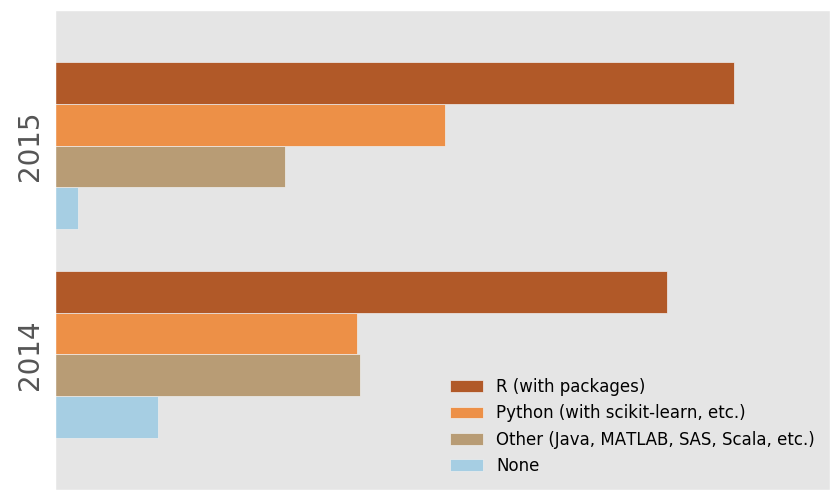
\includegraphics[width=15cm]{figuras/poll-lang}}
	}{
		\Fonte{KDNuggets 2015 poll: Primary programming language for Analytics, Data Mining, Data Science tasks}
	}	
\end{figure}

Além das linguagens e suas bibliotecas citadas, exitem alguns frameworks muito usados pela comunidade de engenheiros de machine learning, 
que não necessáriamente utilizam as linguagens mais comuns, os principais são \textbf{Apache Spark} e o \textbf{Apache Hadoop.}

O framework \textbf{Apache Spark} é voltado para processamento de \textbf{Big Data}, feito para ser usual, rápido e para o uso de análises mais
sofisticadas. É um projeto da \textbf{Fundação Apache}, que é uma organização sem fins lucrativos afim de suportar 
projetos com código livre, logo o \textbf{Spark} é um projeto de código livre. Este vem sendo desenvolvido desde 2009 pelo 
AMPLab da Universidade de Califórnia em Berkeley e em 2010 seu código foi aberto como projeto da fundação Apache. 
O Spark é um framework consolidado que oferece formas de gerenciar e processar Big Data com varias naturezas de dados, como textos ou imagens, e várias origens,  
como lote ou streaming de dados,  de forma muito compreeendivel. Além de melhorar a performance de aplicações e dar mais produtividade no desenvolvimento
de aplicações em Java, Scala, R e Python. Posto seu foco no alto desempenho Spark possui uma bibliteca chamada \textbf{MLlib} para Machine Learning a qual 
consiste nos algoritmos de Machine Learning, como classificação, regressão e clustering.

Assim como o Spark o \textbf{Apache Hadoop} nasceu com a necessidade de processar uma grande quantidade de Big Data e tambem é um \textit{software} 
livre com o código aberto, porém originou-se do framework \textbf{MapReduce} da Google  criado para indexar páginas web, porém foi muito mais além 
, e é utilizado por industrias das áreas de entreterimento, mercado financeiro, governamentais, saúde, informação e outras. Basicamente ele utilza
técnicas do MapReduce para consultar dados e dividir e processa-los paralelamente em vários computadores, oque permite processar muito mais dados em menos
tempo. Assim como o Hadoop o Spark também estende funcionalidades do MapReduce.
 

\subsection{Principais ferramentas}
\label{subsec:ferramentas}
Muitas vezes não é necessáro desenvolver um sitema de machine learning para que se obtenha resultados satisfátórios, pois existem
ferramentas focadas em automatizar algumas tarefas para fazer \textit{data-mining}, preparar os dados ou visualiza-los de formas mais 
simples, além de ferramentas que facilitam o desenvolvimento de algortimos. Existem muitas empresas muito consolidadas no mercado 
que fornecem este tipo de ferramenta como a \textbf{IBM}, \textbf{Oracle} e \textbf{SAP}, no entando a comunidade de desenvolvedores
produzem ótimas ferramentas gratuitas e de código aberto, portanto é aconselhavél que antes de comprar uma ferramenta deste tipo
avaliar se as opções gratuitas não atendem as necessidades, sabendo que os produtos proprietários são relativamente caros. Por 
isto podemos categorizar estas ferramentas como \textbf{pagas} e \textbf{gratuitas}.


Dentre as soluções pagas, é importante citar algumas das principais:

\begin{alineas}
	\item \textbf{IBM SPSS Statistics}, é um pacote de soluções para análises de dados, possui mais de 10 módulos integrados para 
	atender todo o processo de análise desde o planejamento e a coleta dos dados até a análise. Muitos destes módulos são focados na análise
	preditiva, por exemplo com os dados que existente é possivel manter todo um \textit{workflow} de machine learning, para identificar padrões e relações 
	inesperadas;

	\item \textbf{SAP Predictive Analytics}, como apresentado anteriormente antes de aplicar algoritmos que analisem e gerem modelos estatisticos, deve-se 
	preparar os dados, ou seja transformar os dados em uma forma que possa ser processado, pode ser uma tarefa repetitiva, massante e passível de erro humano, 
	vendo isto está ferramenta automatiza estas etapas. Esta ferramenta é capaz de utilziar dados de diversas origens como aplicações, 
	\textit{data warehouses}\footnote{\textbf{Data warehouses} é um armazen de dados históricos de trasações de uma dada empresa, com intuito de criar relatórios para que
	se possa tomar decisões} e até mesmos de arquivos \textit{flats}\footnote{Um arquivo formado de registros do mesmo tipo, sem que 
	exista uma estrutura interna definindo as relações entre os registros.}. 
	Além de fornecer formas de explorar os dados visualmente, tornando mais eficiente a visualização dos resultados, como por exemplo a visualização 
	do tamanho dos \textit{clusters}, densidade, distância, árvores de decisões entre outros. Permite também que se utilize scripts customizados 
	esritos na linguagem \textbf{R}; e

	\item \textbf{SAS Analytics Suite}, é basicamente um ecosistemas de produtos focados em atender todas as etapas de machine learning, como a preparação
	dos dados, visualização dos dados e gerenciamento dos modelos gerados. Além de ser integrada as linguagens R e Python também se intergra com o framework
	Hadoop.	
\end{alineas}

E dentre as soluções abertas e gratuitas, algumas das principais são:

\begin{alineas}
	\item \textbf{RapidMiner}: é um software livre que atende todas as etapas do \textit{workflow} de machine learning, desde a preparação dos dados até 
	a operacionalização em ambiente de produção, em suma em um único ambiente é possivel melhorar drasticamente a performance e eficiência;

	\item \textbf{Weka}: possui uma coleção de algoritmos de machine learning e estes podem ser aplicados diretamente em um conjunto de dados, tembé permite
	que aplicações Java utilizem estes algoritmos, também possui ferramentas para preparação dos dados, classificação, regressão, clusterização e visualização.
	Este é um software sobre a licensa \textbf{GNU}(\textit{General Public License}), é uma das licensas de softwares abertos mais permissivas. 
	Além de possuir uma interface gráfica muito intuitiva que praticamente dispensa a escrita de código, tornando o processo muito mais amigável e
	convidativo para profissionais de diversas áreas; e

	\item \textbf{Rattle}: sabendo que a linguagem R atende o universo de machine learning muito bem por conta das inumeras bibliotecas, porém 
	seu desenvolvimento e visualização dos resultados é em console de linha de comando. A ferrementa Rattle possibilita executar os algoritmos
	em R em uma interface gráfica e visualizar o resultado dos algoritmos gráficamente.	  
\end{alineas}


\subsection{Serviços na nuvem}
\label{subsec:servicos}
Além de ferramentas e as linguagens de programação existem alguns serviços na nuvem que abstraem muita complexidade de um projeto de machine learning, 
desde \textbf{API's}\footnote{\textbf{API} é uma interface para programação de aplicações} para processamento dos dados até serviços de infraestrutura como máquinas com grande poder computacional.
Alguns serviços chegam a oferecer um \textit{setup} interativo que possibilita configurar todo o processo de machine learning em uma interface
simples e de forma visual, ou seja sem linha de comando ou programação.


Os principais fornecedores destes tipos de serviço são pioneiros em serviços de nuvem, são eles \textbf{Microsoft Azure} \textbf{AWS (Amazon Web Services)}, 
ambos possuem soluções de \textbf{IaaS (Infraestrutura como Serviço)}, \textbf{PaaS (Plataforma como Serviço)} e \textbf{SaaS (Software como Serviço)}, e também
possuem serviços focados em machine learning. São eles:

\begin{alineas}
	\item \textbf{Amazon Machine Learning} é baseado nas mesmas tecnologias utilizadas e comprovadas pela própria Amazon, uma empresa que sempre teve vários
	desafios em relação a escalabilidade e performance. Este produto oferce ferramentas para configurar todo o processo de ML de forma simples, não necessitando 
	de muito conhecimento nos algoritmos complexos de ML, após a conclusão dos modelos o serviço oferece API's simples para obter predições apartir dos modelos gerados.
	Porem possui alguns recursos que permitem o usuário identificar se os dados possuem erros ou ruídos, como campos vazios com valores inesperados, para que se possa 
	garantir a precisão do modelo, além dos algoritmos utilizados estarem preparados para garantir a qualidade dos modelos.       
	
	\item \textbf{Azure Machine Learning} oferece praticamente os mesmos recursos que o \textbf{Amazon ML}, 
	além de várias API's online para reconhecimento	facial, moderação de conteúdo, reconhecimento de fala, reconhecimento de voz, tradução, recomendações, entre outras. 
	A maioria destas API's são focada em uma melhor experiência para os usuáros das aplicações que a consomem, por exemplo  recomendação de alguma ação baseda em 
	ações passadas.

	\item \textbf{HPE Haven onDemand} é uma plataforma focada em API's altamente escaláveis para atender qualquer tipo apicação sob demanda,
	 criado pela \textbf{HP Enterprise} e hospedado na nuvem da \textbf{Microsoft Azure}.    	
\end{alineas}







